\begin{center}
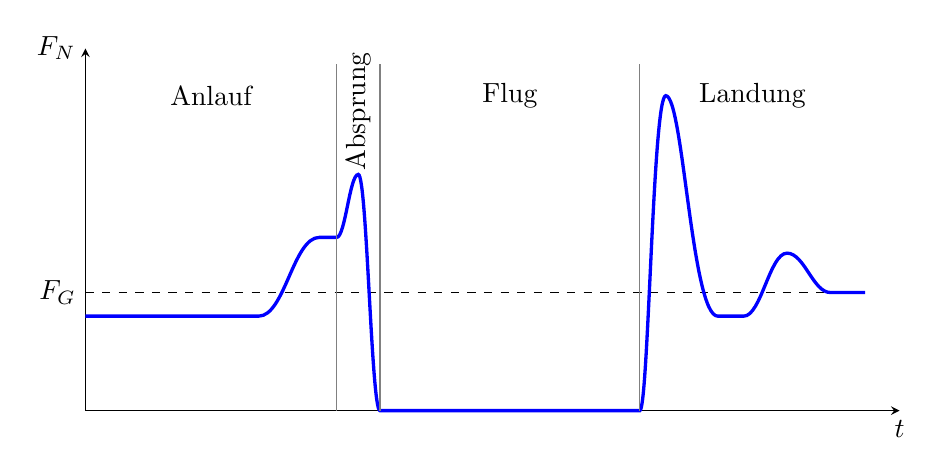
\begin{tikzpicture}[>=stealth, xscale=1.1]
 \draw[->] (0,0) -- (9.4,0) node[below] {$t$};
 \draw[->] (0,0) -- (0,4.6) node[left] {$F_\text{N}$};
 \draw[dashed] (0,1.5) -- (9,1.5);
 \node[left] at (0,1.5) {$F_\text{G}$};
 \draw[blue, very thick] (0,1.2) -- (2,1.2) .. controls (2.3,1.2) and (2.4,2.2) .. (2.7,2.2) -- (2.9,2.2) .. controls (3.0,2.2) and (3.05,3.0) .. (3.15,3.0) .. controls (3.25,3.0) and (3.3,0) .. (3.4,0) -- (6.4,0) .. controls (6.5,0) and (6.55,4.0) .. (6.7,4.0) .. controls (6.9,4.0) and (7.0,1.2) .. (7.3,1.2) -- (7.6,1.2) .. controls (7.8,1.2) and (7.9,2.0) .. (8.1,2.0) .. controls (8.3,2.0) and (8.4,1.5) .. (8.6,1.5) -- (9,1.5);
 \foreach \x in {2.9,3.4,6.4} \draw[gray] (\x,0) -- (\x,4.4);
 \node at (1.45,4.0) {Anlauf};
 \node[rotate=90] at (3.15,3.8) {Absprung};
 \node at (4.9,4.0) {Flug};
 \node at (7.7,4.0) {Landung};
\end{tikzpicture}
\end{center}

\begin{itemize}
\item \emph{Anlauf:} Auf der geneigten Anlaufspur drückt der Springer nur mit der Komponente der Gewichtskraft senkrecht zur Bahn, $F_\text{N} = F_\text{G}\cos\alpha < F_\text{G}$. Im gekrümmten Übergang am Ende der Anlaufspur wird die Normalkraft grösser, weil der Springer auf eine Kreisbahn gezwungen wird.
\item \emph{Absprung:} Der Springer stösst sich kurz und kräftig vom Schanzentisch ab, die Normalkraft hat ein kurzes Maximum.
\item \emph{Flug:} Kein Kontakt mit dem Boden, $F_\text{N} = 0$.
\item \emph{Landung:} Beim Aufsetzen wird die Geschwindigkeit senkrecht zum Hang abgebremst, die Normalkraft hat ein hohes, kurzes Maximum. Danach ist sie am steilen Hang wieder kleiner als $F_\text{G}$, steigt im Auslauf (gekrümmter Übergang) nochmals an und ist im flachen Auslauf gleich $F_\text{G}$.
\end{itemize}
